\documentclass{standalone}
\usepackage{pgfplots}
\pgfplotsset{compat=1.18}
\usepackage{amsmath}
\usetikzlibrary{decorations, decorations.text,backgrounds}

\begin{document}
	
	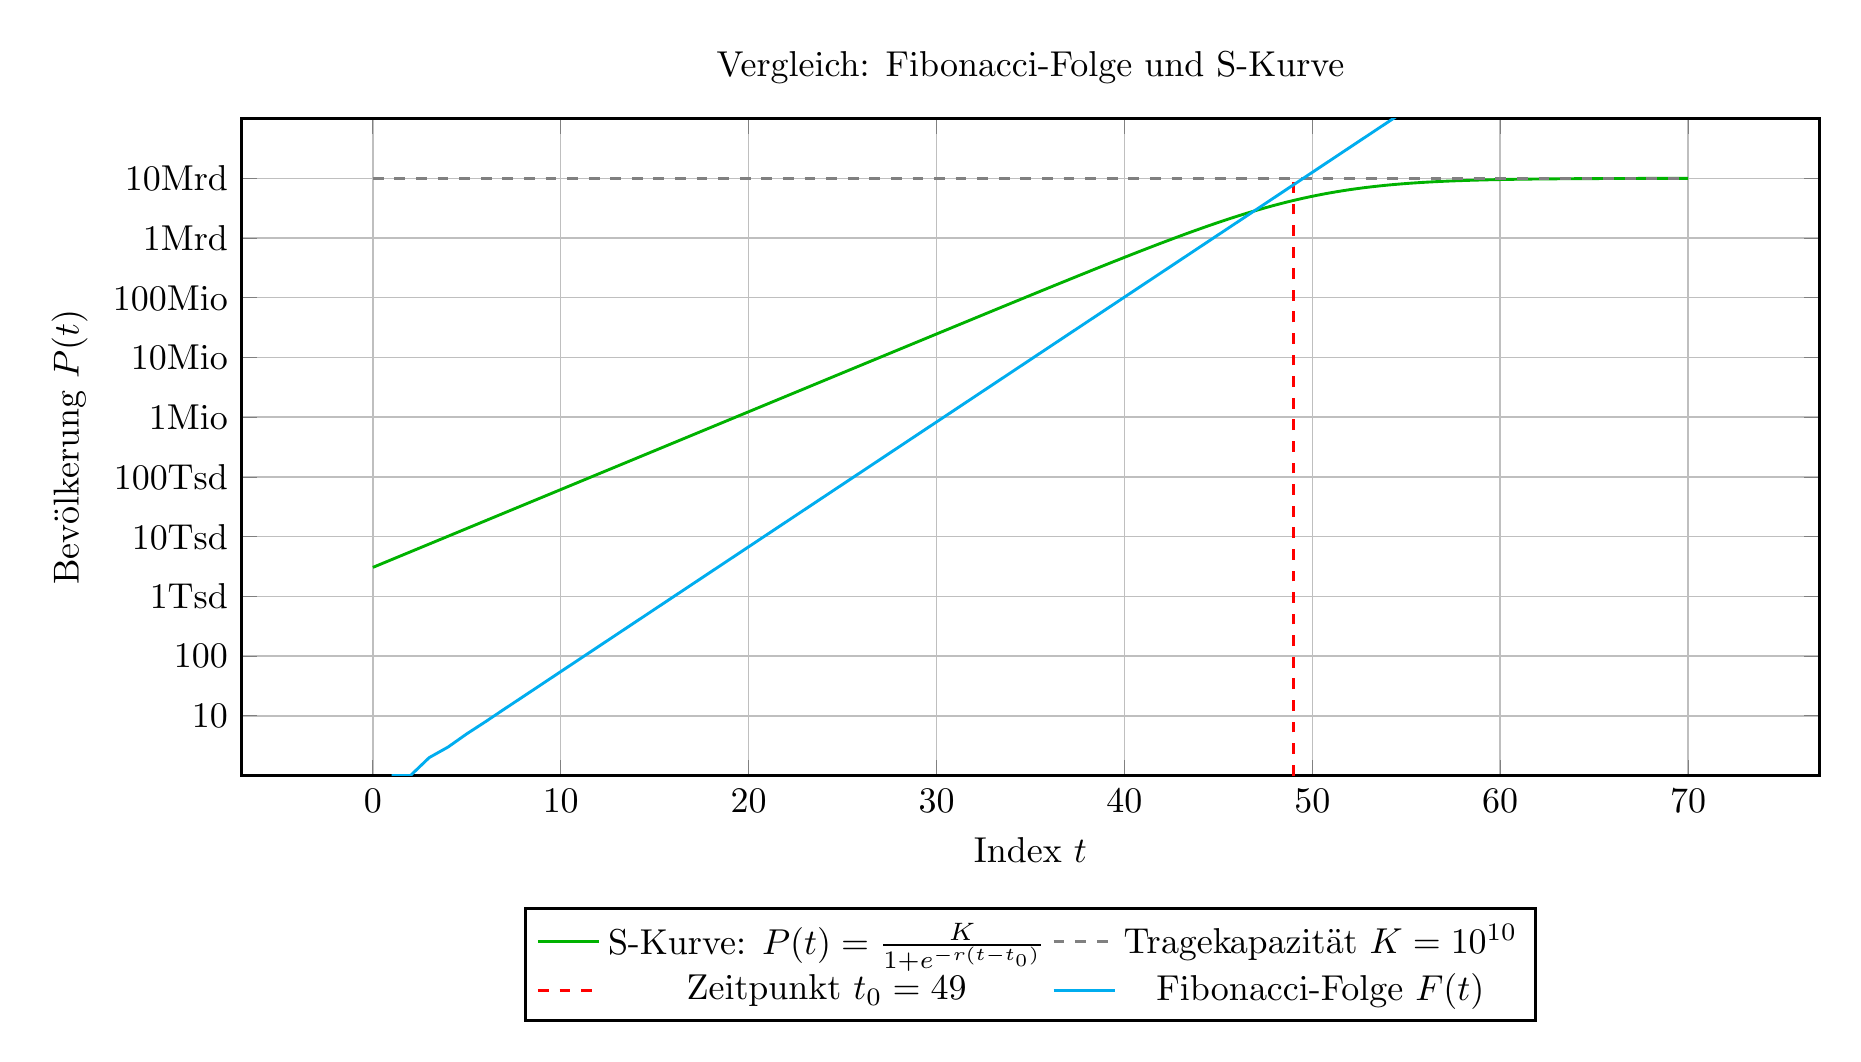
\begin{tikzpicture}[background rectangle/.style={fill=white}, show background rectangle, scale=1.3]
		\begin{semilogyaxis}[
			width=17cm,
			height=8cm,
			xlabel={Index $t$},
			ylabel={Bevölkerung $P(t)$},
			title={Vergleich: Fibonacci-Folge und S-Kurve},
			grid=both,
			ymin=1,
			ymax=1e11,
			xtick={0,10,...,70},
			ytick={1e1,1e2,1e3,1e4,1e5,1e6,1e7,1e8,1e9,1e10},
			yticklabels={10,100,1Tsd,10Tsd,100Tsd,1Mio,10Mio,100Mio,1Mrd,10Mrd},
			legend style={at={(0.5,-0.2)}, anchor=north, legend columns=2},
			log basis y=10,
			thick
			]
			
			% S-Kurve: logistische Funktion
			\addplot[
			green!70!black,
			domain=0:70,
			samples=300,
			thick
			] {1e10 / (1 + exp(-0.3*(x - 50)))};
			\addlegendentry{S-Kurve: $P(t) = \frac{K}{1 + e^{-r(t - t_0)}}$}
			
			% Tragekapazität
			\addplot [gray, dashed, domain=0:70] {1e10};
			\addlegendentry{Tragekapazität $K = 10^{10}$}
			
			% Zeitpunkt bei t = 50
			\addplot [red, dashed] coordinates {(49,1e0) (49,1e10)};
			\addlegendentry{Zeitpunkt $t_0 = 49$}
			
			% Fibonacci-Folge als Punkte
			\addplot[
			cyan
			] coordinates {
				(0,0)
				(1,1)
				(2,1)
				(3,2)
				(4,3)
				(5,5)
				(6,8)
				(7,13)
				(8,21)
				(9,34)
				(10,55)
				(11,89)
				(12,144)
				(13,233)
				(14,377)
				(15,610)
				(16,987)
				(17,1597)
				(18,2584)
				(19,4181)
				(20,6765)
				(21,10946)
				(22,17711)
				(23,28657)
				(24,46368)
				(25,75025)
				(26,121393)
				(27,196418)
				(28,317811)
				(29,514229)
				(30,832040)
				(31,1346269)
				(32,2178309)
				(33,3524578)
				(34,5702887)
				(35,9227465)
				(36,14930352)
				(37,24157817)
				(38,39088169)
				(39,63245986)
				(40,102334155)
				(41,165580141)
				(42,267914296)
				(43,433494437)
				(44,701408733)
				(45,1134903170)
				(46,1836311903)
				(47,2971215073)
				(48,4807526976)
				(49,7778742049)
				(50,12586269025)
				(51,20365011074)
				(52,32951280099)
				(53,53316291173)
				(54,86267571272)
				(55,139583862445)
				(56,225851433717)
				(57,365435296162)
				(58,591286729879)
				(59,956722026041)
				(60,1548008755920)
				(61,2504730781961)
				(62,4052739537881)
				(63,6557470319842)
				(64,10610209857723)
				(65,17167680177565)
				(66,27777890035288)
				(67,44945570212853)
				(68,72723460248141)
				(69,117669030460994)
				(70,190392490709135)
			};
			\addlegendentry{Fibonacci-Folge $F(t)$}
			
		\end{semilogyaxis}
	\end{tikzpicture}
	
\end{document}
